\section{标准化波动}
\label{sec:clt-standardized}

掷$n$次硬币，我们可以看正面次数$S_n$，也可以看正面比例$\bar{X}_n=S_n/n$。两者只差一个因子$n$，可是随着$n$增大，一个越来越分散，一个越来越集中。要谈“波动的形状”，先得说清楚三件事：以什么为中心，看哪一个误差量，把误差放大多少倍。

第~\ref{chap:laws-of-large-numbers}章的大数律回答了中心的问题：样本平均趋于总体均值$\mu$，平均的偏差$\bar{X}_n-\mu$趋于零。它没有回答偏差以多快的速度缩小，也没有说明把偏差放大到合适的倍数以后是什么样子。本节先用方差确定合适的放大倍数，再说明标准化能做到什么、做不到什么。

\subsection{部分和与平均的尺度}
\label{sec:clt-scales}

设$X_1,X_2,\dots$独立同分布，均值为$\mu$，方差$\sigma^2$有限且大于零。记部分和与样本平均为
\[
 S_n=X_1+\dots+X_n,\qquad \bar{X}_n=\frac{S_n}{n} .
\]
两种误差量分别是部分和偏离$n\mu$的量$S_n-n\mu$，以及平均偏离$\mu$的量$\bar{X}_n-\mu$。

\paragraph{两种误差的方差}
独立随机变量之和的方差等于方差之和，常数平移不改变方差，所以
\[
 \operatorname{Var}(S_n-n\mu)=\sum_{i=1}^{n}\operatorname{Var}(X_i)=n\sigma^2 .
\]
再利用$\operatorname{Var}(aY)=a^2\operatorname{Var}(Y)$，取$a=1/n$，得到
\[
 \operatorname{Var}(\bar{X}_n-\mu)=\frac{1}{n^2}\cdot n\sigma^2=\frac{\sigma^2}{n} .
\]
两个结果合起来，标准差分别是
\begin{equation}
 \sqrt{\operatorname{Var}(S_n-n\mu)}=\sigma\sqrt{n},\qquad
 \sqrt{\operatorname{Var}(\bar{X}_n-\mu)}=\frac{\sigma}{\sqrt{n}} .
 \label{eq:clt-scales}
\end{equation}

部分和的典型偏差随$\sqrt{n}$增长，比$n$慢；平均的典型偏差随$1/\sqrt{n}$缩小，比$1/n$慢。前者慢于$n$，是因为独立的正负偏差互相抵消了一部分；后者慢于$1/n$，原因相同。把$n$项完全同向的偏差相加，标准差才会是$n\sigma$。

\paragraph{掷硬币}
设$X_i\sim\operatorname{Bern}(1/2)$，则$\mu=1/2$，$\sigma^2=1/4$，$S_n\sim\operatorname{Bin}(n,1/2)$。由式~\eqref{eq:clt-scales}，次数与比例的标准差分别为$\sqrt{n}/2$与$1/(2\sqrt{n})$。取$n=10,40,160$，
\[
 \frac{\sqrt{n}}{2}\approx1.58,\ 3.16,\ 6.32;\qquad \frac{1}{2\sqrt{n}}\approx0.158,\ 0.079,\ 0.040 .
\]
$n$每变成四倍，次数的标准差加倍，比例的标准差减半。

图~\ref{fig:clt-binomial-scales}画出这三个$n$下的精确质量表。左图以$n/2$为中心看次数，质量表随$n$摊开，峰值下降；右图以$1/2$为中心看比例，质量表向中心收拢。为了让不同$n$可比，右图的纵轴是质量除以格点间距$1/n$，这样曲线下的面积都是一。

\begin{BookInlineFigure}
 \centering
 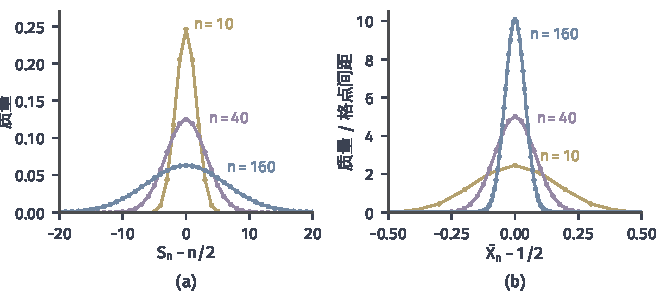
\includegraphics[width=112mm]{figures/07-probability/03-probability-limits/matplotlib/clt-binomial-scales/figure.pdf}
 \caption{均匀硬币掷$n$次的正面次数$S_n\sim\operatorname{Bin}(n,1/2)$，$n=10$（黄）、$40$（紫）、$160$（蓝），折线连接各格点上的精确质量。(a)中心化次数$S_n-n/2$的质量，宽度按$\sqrt{n}/2$增长；(b)中心化比例$\bar{X}_n-1/2$的质量除以格点间距$1/n$，宽度按$1/(2\sqrt{n})$缩小。}
 \label{fig:clt-binomial-scales}
\end{BookInlineFigure}

\paragraph{两种尺度不能混用}
这两个量回答不同的问题。问“正面次数偏离$n/2$不超过$5$次的概率”，随着$n$增大，这个概率趋于零，因为次数的典型偏差$\sqrt{n}/2$终将远超$5$。问“正面比例偏离$1/2$不超过$0.05$的概率”，它趋于一，这是大数律。两句话都对，只是固定的容许量$5$与$0.05$放在了不同的尺度上。

\paragraph{放大的倍数}
要得到不随$n$消失、也不随$n$发散的波动，可以把平均的偏差乘以$n^{a}$，看哪个$a$合适。由$\operatorname{Var}(cY)=c^2\operatorname{Var}(Y)$，
\[
 \operatorname{Var}\bigl(n^{a}(\bar{X}_n-\mu)\bigr)=n^{2a}\cdot\frac{\sigma^2}{n}=n^{2a-1}\sigma^2 .
\]
$a<1/2$时方差趋于零，由Chebyshev不等式，对每个$t>0$，
\[
 \mathbb{P}\bigl(\lvert n^{a}(\bar{X}_n-\mu)\rvert\geq t\bigr)\leq\frac{n^{2a-1}\sigma^2}{t^2}\to0 ,
\]
放大后的偏差依概率趋于零，形状缩成一点。$a>1/2$时方差趋于无穷，偏差越放越大。只有$a=1/2$时方差恒为$\sigma^2$。

图~\ref{fig:clt-three-scalings}用掷硬币的精确分布画出$a=0.3,0.5,0.7$三种放大下，中间$90\%$质量所在的区间随$n$的变化。三幅图的区间分别收窄、保持、扩张，紫色虚线是按方差预测的$\pm1.645\cdot\frac12 n^{a-1/2}$，其中$1.645$是标准高斯分布的$95\%$分位数。$a=1/2$时区间端点稳定在$\pm0.82$附近，与这条虚线吻合，这已经在提示极限分布是高斯的。

\begin{BookInlineFigure}
 \centering
 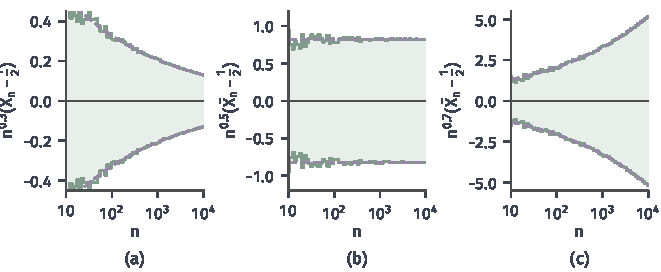
\includegraphics[width=112mm]{figures/07-probability/03-probability-limits/matplotlib/clt-three-scalings/figure.pdf}
 \caption{掷硬币时$n^{a}(\bar{X}_n-1/2)$的$5\%$与$95\%$分位数（绿色阶梯，由$\operatorname{Bin}(n,1/2)$精确计算），$n$从$10$到$10^{4}$，横轴为对数刻度。(a)$a=0.3$；(b)$a=0.5$；(c)$a=0.7$。紫色虚线为$\pm1.645\cdot\frac12n^{a-1/2}$。}
 \label{fig:clt-three-scalings}
\end{BookInlineFigure}

\paragraph{大数律与中心极限的分工}
大数律相当于取$a=0$：平均的偏差本身趋于零，它确定了极限的位置。中心极限定理研究$a=1/2$时放大后偏差的分布。前者不能推出后者：知道偏差趋于零，并不知道它以$1/\sqrt{n}$的速度趋于零，更不知道放大以后呈什么形状。下一小节会看到，平均同样趋于中心，放大后的形状却可以不是钟形。

方差无穷时，式~\eqref{eq:clt-scales}失去意义。例如第~\ref{chap:tail-probabilities}章参数为$3/2$的Pareto分布，均值有限，样本平均仍满足大数律，方差却是无穷，$\sqrt{n}$不再是合适的放大倍数。本章始终假设方差有限，这类重尾的极限需要别的尺度，不在本卷讨论。

\subsection{标准化的选择}
\label{sec:clt-standardization}

确定了放大倍数$\sqrt{n}$，再除以单项的标准差，就把波动的单位也去掉了。由式~\eqref{eq:clt-scales}，中心化部分和除以它自己的标准差，与平均的偏差乘$\sqrt{n}$再除以$\sigma$，是同一个量。

\begin{definition}[标准化部分和]
\label{def:clt-standardized-sum}
设$X_1,\dots,X_n$独立同分布，均值为$\mu$，方差$\sigma^2\in(0,\infty)$。称
\begin{equation}
 Z_n=\frac{S_n-n\mu}{\sigma\sqrt{n}}=\frac{\sqrt{n}\,(\bar{X}_n-\mu)}{\sigma}
 \label{eq:clt-zn}
\end{equation}
为标准化部分和。
\end{definition}

$Z_n$正是第~\ref{chap:random-variable-moments}章意义下$S_n$的标准化，也是$\bar{X}_n$的标准化：两者只差一个正的倍数，标准化后相同。由式~\eqref{eq:clt-scales}，对每个$n$都有
\[
 \mathbb{E}[Z_n]=0,\qquad \operatorname{Var}(Z_n)=1 .
\]
掷硬币时$\mu=1/2$，$\sigma=1/2$，于是$Z_n=(2S_n-n)/\sqrt{n}$。$n=100$时$Z_{100}=(S_{100}-50)/5$，章首的阈值$55$对应$Z_{100}=1$。

\paragraph{方差为一不等于钟形}
标准化只做平移和正的缩放，不改变分布的形状。$n=1$时$Z_1$就是$X_1$的标准化，硬币的$Z_1$只取$\pm1$两个值，与钟形毫无关系。$Z_n$接近钟形，是因为$S_n$是许多独立项之和，不是因为除以了标准差。

即使项数很多，标准化也不能保证钟形。设第$n$次试验掷$n$枚特制的硬币，每枚正面的概率是$1/n$，正面总数$S_n\sim\operatorname{Bin}(n,1/n)$。它的均值和方差是
\[
 \mathbb{E}[S_n]=1,\qquad \operatorname{Var}(S_n)=n\cdot\frac1n\Bigl(1-\frac1n\Bigr)=1-\frac1n .
\]
平均$S_n/n$同样趋于零，标准化以后均值为零、方差为一。可是$S_n$只取非负整数，它的前几个质量趋于
\[
 \mathbb{P}(S_n=0)=\Bigl(1-\frac1n\Bigr)^{n}\to\mathrm{e}^{-1}\approx0.368,\qquad
 \mathbb{P}(S_n=1)=\Bigl(1-\frac1n\Bigr)^{n-1}\to\mathrm{e}^{-1} .
\]
一般地，第~\ref{chap:common-distributions}章已经说明$\operatorname{Bin}(n,\lambda/n)$的质量趋于$\operatorname{Poisson}(\lambda)$的质量，这里$\lambda=1$，所以$S_n-1$的分布逼近$\operatorname{Poisson}(1)$平移$-1$后的分布。

图~\ref{fig:clt-poisson-counter}把这两种标准化计数放在一起。左边是$\operatorname{Bin}(100,1/2)$，格点间距$1/5$，质量除以间距后贴着标准高斯密度$\varphi$；右边是$\operatorname{Bin}(100,1/100)$，标准化以后只有几根竖线，集中在$z=-1,0,1,2$附近，没有平滑的钟形。

\begin{BookInlineFigure}
 \centering
 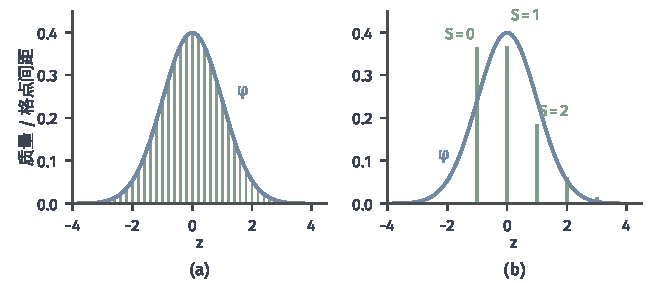
\includegraphics[width=112mm]{figures/07-probability/03-probability-limits/matplotlib/clt-poisson-counter/figure.pdf}
 \caption{两个$n=100$的标准化二项计数，均值都为$0$、方差都为$1$。绿色竖线是精确质量除以格点间距$1/\sigma_n$，蓝线是标准高斯密度$\varphi$。(a)$\operatorname{Bin}(100,1/2)$，$\sigma_n=5$；(b)$\operatorname{Bin}(100,1/100)$，$\sigma_n\approx0.995$，质量集中在$S=0,1,2$等少数格点。}
 \label{fig:clt-poisson-counter}
\end{BookInlineFigure}

两种计数的差别在于每一项对总和的影响。正面概率为$1/2$时，每枚硬币只贡献总方差的$1/n$，没有哪一枚举足轻重；正面概率为$1/n$时，总和几乎由“偶尔出现的一次正面”决定，这样一次正面就让$S_n$跳动一个标准差。第~\ref{sec:clt-non-identical}节会把“没有一项举足轻重”写成可以核验的条件。

\paragraph{零方差}
定义~\ref{def:clt-standardized-sum}要求$\sigma^2>0$。若$\sigma^2=0$，则$X_i$以概率一等于$\mu$，部分和$S_n-n\mu$以概率一为零，没有波动可言，也不能除以$\sigma$。此时不作标准化，直接说$\sqrt{n}(\bar{X}_n-\mu)$以概率一等于零，它的分布是$0$处的单点分布。把方差为零的高斯分布$\mathcal{N}(0,0)$理解为这个单点分布，零方差情形也可以纳入第~\ref{sec:clt-multivariate}节的统一陈述。
